\documentclass[twocolumn,landscape]{amsart}

\usepackage[nopdftoc]{lymber}
\usepackage{enumerate}

\usepackage[T1]{fontenc}
\usepackage{textcomp}
\usepackage{mathpazo}
\usepackage{utopia}
\usepackage{graphicx}

\usepackage[cm]{fullpage}

\renewcommand{\arraystretch}{1.5}

\begin{document}

\twocolumn[\begin{@twocolumnfalse}
  \titulo{FUVEST 2013 --- Algumas questões}
  \subtitulo{Extraído para testar o gerador de provas.}

\begin{tabular}{llll}
  {\bf Nome:}&\underline{\hspace{15cm}}&{\bf NUSP:}&\underline{\hspace{5cm}}\\
  &&&\\
  {\bf Professor:}&\underline{\hspace{15cm}}&{\bf Turma:}&\underline{\hspace{5cm}}\\
\end{tabular}

\vspace{1cm}

\section*{Instruções}

\begin{enumerate}
  \item A prova tem início às 7:30h e duração de 2 horas.
  \item Não é permitido deixar a sala sem entregar a prova.
  \item Todo material não necessário à prova (mochilas, bolsas,
  calculadoras, agasalhos, bonés, celulares, livros, etc.) deve ficar na
  frente da sala.
  \item Sobre a carteira deve permanecer apenas lápis, caneta, borracha
  e documento de identidade com foto.
  \item É permitida a entrada na sala até às 8:00h e não é permitida a
  saída da sala antes das 8:10h.
  \item As respostas devem ser transferidas para a folha óptica durante
  as 2 horas de prova (não há tempo extra para o preenchimento da folha
  óptica).
  \item Só destaque o gabarito do aluno (última folha) quando for
  entregar a prova. Não esqueça de anotar o tipo de prova no gabarito do
  aluno (para que você possa depois conferir suas respostas com o
  gabarito oficial).
  \item A folha óptica deve ser preenchida com caneta esferográfica azul
  ou preta.
  \item Para o correto preenchimento da folha óptica siga o exemplo
  abaixo.
\end{enumerate}

\end{@twocolumnfalse}]

\begin{figure}[h!]
  \centering
  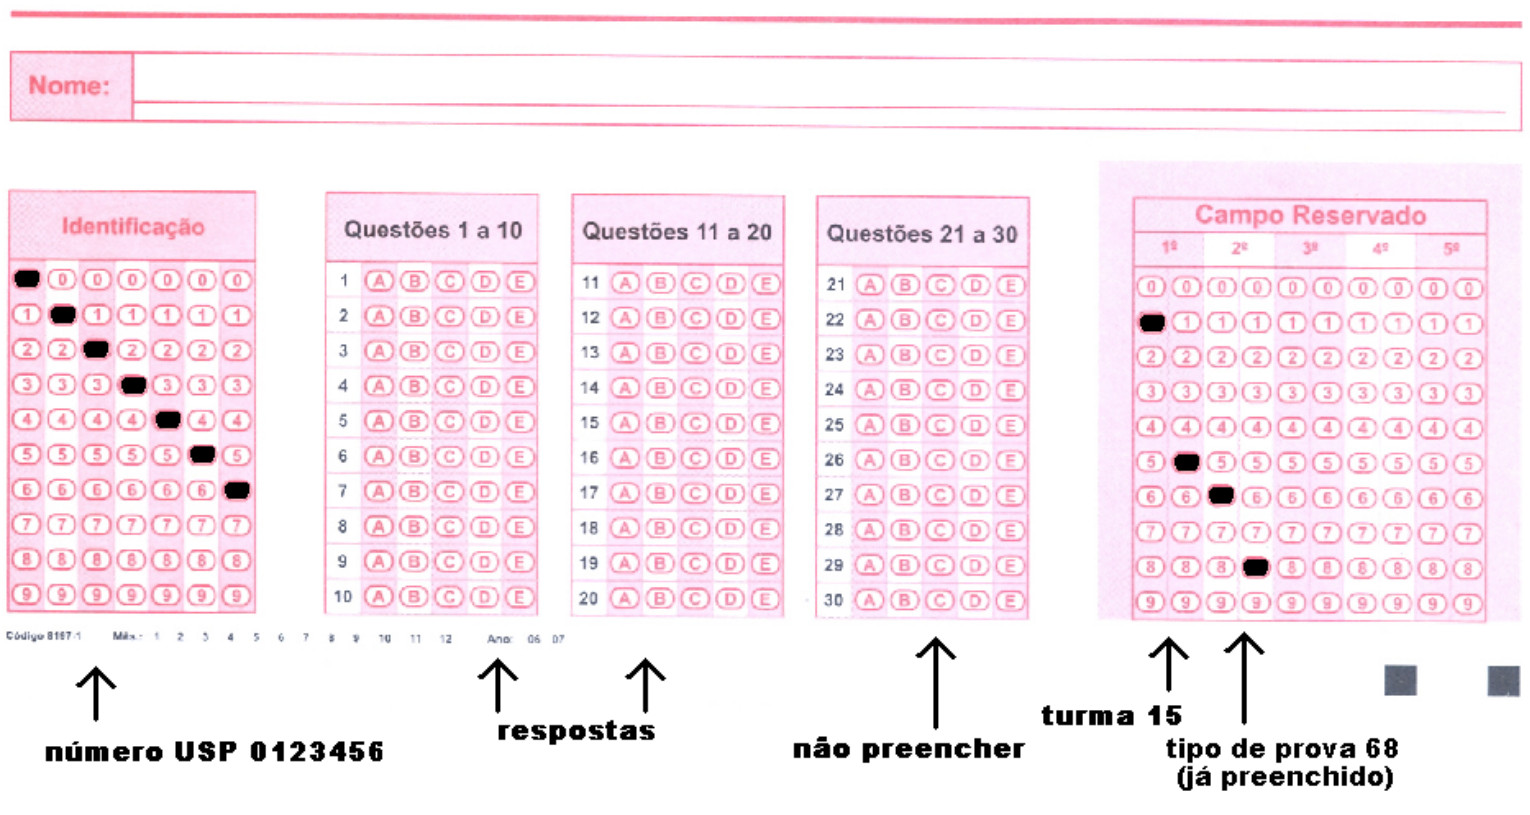
\includegraphics[width=12cm]{front-gabarito.jpg} % para gerar pdf    
\end{figure}

\thispagestyle{empty}

\cleardoublepage

\begin{questao}
  Vinte times de futebol disputam a Série A do Campeonato Brasileiro,
  sendo seis deles paulistas.  Cada time joga duas vezes contra cada um
  dos seus adversários. A porcentagem de jogos nos quais os dois
  oponentes são paulistas é
  \begin{enumerate}[\bf a.]
    \item menor que 7\%.
    \item maior que 7\%, mas menor que 10\%. %%% correta
    \item maior que 10\%, mas menor que 13\%.
    \item maior que 13\%, mas menor que 16\%.
    \item maior que 16\%.
  \end{enumerate}
\end{questao}
\clearpage

\begin{questao}
  São dados, no plano cartesiano, o ponto $P$ de coordenadas $(3,6)$ e a
  circunferência $C$ de equação $(x-1)^2+(y-2)^2=1$. Uma reta $t$ passa
  por $P$ e é tangente a $C$ em um ponto $Q$. Então a distância de $P$ a
  $Q$ é

  \begin{enumerate}[\bf a.]
    \item $\sqrt{15}$.
    \item $\sqrt{17}$.
    \item $\sqrt{18}$.
    \item $\sqrt{19}$. %%% correta
    \item $\sqrt{20}$.
  \end{enumerate}
\end{questao}
\clearpage

\begin{questao}
  Os vértices de um tetraedro regular são também vértices de um cubo de
  aresta 2. A área de uma face desse tetraedro é

  \begin{enumerate}[\bf a.]
    \item $2\sqrt{3}$. %%% correta
    \item 4.
    \item $3\sqrt{2}$.
    \item $3\sqrt{3}$.
    \item 6.
  \end{enumerate}
\end{questao}
\clearpage

\begin{questao} 
  Sejam $\alpha$ e $\beta$ números reais com
  $-\frac{\pi}{2}\leq\alpha\leq\frac{\pi}{2}$ e $0\leq\beta\leq\pi$ . Se o
  sistema de equações, dado em notação matricial, \[
  \begin{bmatrix}
    3&6\\
    6&8
  \end{bmatrix}
  \begin{bmatrix}
    \tan\alpha\\\cos\beta
  \end{bmatrix} =
  \begin{bmatrix}
    0\\-2\sqrt{3}
  \end{bmatrix}\] for satisfeito, então $\alpha+\beta$ é igual a

  \begin{enumerate}[\bf a.]
    \item $-\frac{\pi}{3}$.
    \item $-\frac{\pi}{6}$. %%% correta
    \item $0$.
    \item $\frac{\pi}{6}$.
    \item $\frac{\pi}{3}$.
  \end{enumerate}
\end{questao}
\clearpage

\begin{questao}
  As propriedades aritméticas e as relativas à noção de ordem
  desempenham um importante papel no estudo dos números reais. Nesse
  contexto, qual das afirmações abaixo é correta?
  \begin{enumerate}[\bf a.]
    \item Quaisquer que sejam os números reais positivos $a$ e $b$, é
    verdadeiro que $\sqrt{a+b}=\sqrt{a}+\sqrt{b}$.
    \item Quaisquer que sejam os números reais $a$ e $b$ tais que
    $a^2-b^2=0$, é verdadeiro que $a=b$.
    \item Qualquer que seja o número real $a$, é verdadeiro que
    $\sqrt{a^2}=a$.
    \item Quaisquer que sejam os números reais $a$ e $b$ não nulos tais
    que $a<b$, é verdadeiro que $\frac{1}{a}<\frac{1}{b}$.
    \item Qualquer que seja o número real $a$, com $0<a<1$, é verdadeiro
    que $a^2<\sqrt{a}$. %%% correta
  \end{enumerate}
\end{questao}
\clearpage

\begin{questao}
  A extremidade de uma fibra ótica adquire o formato arredondado de uma
  microlente ao ser aquecida por um laser, acima da temperatura de
  fusão. A figura abaixo ilustra o formato da microlente para tempos de
  aquecimento crescentes ($t_1<t_2<t_3$).

  Considere as afirmações:

  \begin{enumerate}[\bf I.]
    \item O raio de curvatura da microlente aumenta com
    tempos crescentes de aquecimento.
    \item A distância focal da microlente diminui com tempos
    crescentes de aquecimento.
    \item Para os tempos de aquecimento apresentados na
    figura, a microlente é convergente.
  \end{enumerate}

  Está correto apenas o que se afirma em

  \begin{enumerate}[\bf a.]
    \item I.
    \item II.
    \item III.
    \item I e III.
    \item II e III. %%% correta
  \end{enumerate}
\end{questao}
\clearpage

\begin{questao}
  Quando se divide o Produto Interno Bruto (PIB) de um país pela sua
  população, obtém-se a renda per capita desse país. Suponha que a
  população de um país cresça à taxa constante de 2\% ao ano e que
  $\sqrt[20]{2}\approx 1,035$. Para que sua renda per capita dobre em 20
  anos, o PIB deve crescer anualmente à taxa constante de,
  aproximadamente,
  \begin{enumerate}[\bf a.]
    \item 4,2\%;
    \item 5,6\%; %%% correta
    \item 6,4\%;
    \item 7,5\%;
    \item 8,9\%;
  \end{enumerate}
\end{questao}
\clearpage

\begin{questao}
  O mapa de uma região utiliza a escala de $1:200.000$. A porção desse
  mapa, contendo uma Área de Preservação Permanente (APP), está
  representada na figura, na qual $\overline{AF}$ e $\overline{DF}$ são
  segmentos de reta, o ponto $G$ está no segmento $\overline{AF}$, o
  ponto $E$ está no segmento $\overline{DF}$, $ABEG$ é um retângulo e
  $BCDE$ é um trapézio. Se $\overline{AF}=15$, $\overline{AG}=12$,
  $\overline{AB}=6$, $\overline{CD}=3$ e $\overline{DF}=5\sqrt{5}$
  indicam valores em centímetros no mapa real, então a área da APP é
  \begin{enumerate}[\bf a.]
    \item $100 Km^2$;
    \item $108 Km^2$;
    \item $210 Km^2$;
    \item $240 Km^2$;
    \item $444 Km^2$; %%% correta
  \end{enumerate}
\end{questao}
\clearpage

\begin{questao}
  Seja $f$ uma função a valores reais, com domínio $D\subset\R$, tal que
  $f(x)=\log_{10}\big(\log_{\frac{1}{3}}(x^2-x+1)\big)$ , para todo
  $x\in D$. O conjunto que pode ser o domínio $D$ é
  \begin{enumerate}[\bf a.]
    \item $\{x\in\R: 0<x<1\}$; %%% correta
    \item $\{x\in\R: x\leq 0\mbox{ ou } x\geq 1\}$;
    \item $\{x\in\R: \frac{1}{3}<x<10\}$;
    \item $\{x\in\R: x\leq \frac{1}{3}\mbox{ ou } x\geq 10\}$;
    \item $\{x\in\R: \frac{1}{9}<x<\frac{10}{3}\}$;
  \end{enumerate}
\end{questao}
\clearpage

\begin{questao}
  Frequentemente, os fungos são estudados juntamente com as plantas, na
  área da Botânica. Em termos biológicos, é correto afirmar que essa
  aproximação
  \begin{enumerate}[\bf a.]
    \item não se justifica, pois a organização dos tecidos nos fungos
    assemelha-se muito mais à dos animais que à das plantas.
    \item se justifica, pois as células dos fungos têm o mesmo tipo de
    revestimento que as células vegetais.
    \item não se justifica, pois a forma de obtenção e armazenamento de
    energia nos fungos é diferente da encontrada nas plantas. %%% correta
    \item se justifica, pois os fungos possuem as mesmas organelas
    celulares que as plantas.
    \item se justifica, pois os fungos e as algas verdes têm o mesmo
    mecanismo de reprodução.
  \end{enumerate}
\end{questao}
\clearpage

\begin{questao}
  No morango, os frutos verdadeiros são as estruturas escuras e rígidas
  que se encontram sobre a parte vermelha e suculenta. Cada uma dessas
  estruturas resulta, diretamente,
  \begin{enumerate}[\bf a.]
    \item da fecundação do óvulo pelo núcleo espermático do
    grão de pólen.
    \item do desenvolvimento do ovário, que contém a
    semente com o embrião. %%% correta
    \item da fecundação de várias flores de uma mesma
    inflorescência.
    \item da dupla fecundação, que é exclusiva das
    angiospermas.
    \item do desenvolvimento do endosperma que nutrirá o embrião.
  \end{enumerate}
\end{questao}
\clearpage

\begin{questao}
  A população indígena brasileira aumentou 150\% na década de 1990,
  passando de 294 mil pessoas para 734 mil, de acordo com uma pesquisa
  divulgada pelo Instituto Brasileiro de Geografia e Estatística
  (IBGE). O crescimento médio anual foi de 10,8\%, quase seis vezes
  maior do que o da população brasileira em geral.
  \begin{flushright}
    \url{http://webradiobrasilindigena.wordpress.com, 21/11/2007}.
  \end{flushright}
  A notícia acima apresenta
  \begin{enumerate}[\bf a.]
    \item dado pouco relevante, já que a maioria das populações
    indígenas do Brasil encontra-se em fase de extinção, não
    subsistindo, inclusive, mais nenhuma população originária dos tempos
    da colonização portuguesa da América.
    \item discrepância em relação a uma forte tendência histórica
    observada no Brasil, desde o século XVI, mas que não é uniforme e
    absoluta, já que nas últimas décadas não apenas tais populações
    indígenas têm crescido, mas também o próprio número de indivíduos
    que se autodenominam indígenas.%%% correta
    \item um consenso em torno do reconhecimento da importância dos
    indígenas para o conjunto da população brasileira, que se revela na
    valorização histórica e cultural que tais elementos sempre mereceram
    das instituições nacionais.
    \item resultado de políticas públicas que provocaram o fim dos
    conflitos entre os habitantes de reservas indígenas e demais agentes
    sociais ao seu redor, como proprietários rurais e pequenos
    trabalhadores.
    \item natural continuidade da tendência observada desde a criação
    das primeiras políticas governamentais de proteção às populações
    indígenas, no começo do século XIX, que permitiram a reversão do
    anterior quadro de extermínio observado até aquele momento.
  \end{enumerate}
\end{questao}
\clearpage

\begin{questao}
  A escravidão na Roma antiga
  \begin{enumerate}[\bf a.]
    \item permaneceu praticamente inalterada ao longo dos séculos, mas
    foi abolida com a introdução do cristianismo.
    \item previa a possibilidade de alforria do escravo apenas no caso
    da morte de seu proprietário.
    \item era restrita ao meio rural e associada ao trabalho braçal, não
    ocorrendo em áreas urbanas, nem atingindo funções intelectuais ou
    administrativas.
    \item pressupunha que os escravos eram humanos e, por isso, era
    proibida toda forma de castigo físico.
    \item variou ao longo do tempo, mas era determinada por três
    critérios: nascimento, guerra e direito civil. %%% correta
  \end{enumerate}
\end{questao}
\clearpage

\begin{questao}
  Considere as seguintes substituições propostas para diferentes trechos
  do texto:
  \begin{enumerate}[\bf I.]
    \item ``o número a que chegasse'' (L. 14-15) = o número a
    que alcançasse.
    \item ``Lembro o orgulho'' (L. 18) = Recordo-me do
    orgulho.
    \item ``coisas que deixamos de fazer'' (L. 28-29) = coisas
    que nos descartamos.
    \item ``não há mais bondes'' (L. 31) = não existe mais
    bondes.
  \end{enumerate}
  A correção gramatical está preservada apenas no que foi proposto em
  \begin{enumerate}[\bf a.]
    \item I.
    \item II. %%% correta
    \item III.
    \item II e IV.
    \item I, III e IV.
  \end{enumerate}
\end{questao}
\clearpage

\begin{questao}
  Leia o seguinte texto.

  O autor pensava estar romanceando o processo brasileiro de guerra e
  acomodação entre as raças, em conformidade com as teorias racistas da
  época, mas, na verdade, conduzido pela lógica da ficção, mostrava um
  processo primitivo de exploração econômica e formação de classes, que
  se encaminhava de um modo passavelmente bárbaro e desmentia as ilusões
  do romancista.
  \begin{flushright}
    \emph{Roberto Schwarz}. Adaptado.
  \end{flushright}
  Esse texto crítico refere-se ao livro
  \begin{enumerate}[\bf a.]
    \item Memórias de um sargento de milícias.
    \item Til.
    \item O cortiço. %%% correta
    \item Vidas secas.
    \item Capitães da areia.
  \end{enumerate}
\end{questao}
\clearpage

\begin{questao}
  Em quatro das alternativas abaixo, registram-se alguns dos aspectos
  que, para bem caracterizar o gênero e o estilo das Memórias póstumas
  de Brás Cubas, o crítico J. G. Merquior pôs em relevo nessa obra de
  Machado de Assis. A única alternativa que, invertendo, aliás, o juízo
  do mencionado crítico, aponta uma característica que NÃO se aplica à
  obra em questão é:
  \begin{enumerate}[\bf a.]
    \item ausência praticamente completa de distanciamento enobrecedor
    na figuração das personagens e de suas ações.
    \item mistura do sério e do cômico, de que resulta uma abordagem
    humorística das questões mais cruciais.
    \item ampla liberdade do texto em relação aos ditames da
    verossimilhança.
    \item emprego de uma linguagem que evita chamar a atenção sobre si
    mesma, apagando-se, assim, por detrás da coisa narrada. %%% correta
    \item uso frequente de gêneros intercalados --- por exemplo, cartas ou
    bilhetes, historietas etc. --- embutidos no conjunto da obra
    global.
  \end{enumerate}
\end{questao}
\clearpage

\thispagestyle{empty}
\twocolumn[\begin{@twocolumnfalse}
  \titulo{Gabarito do Aluno}
  \bigskip

  \begin{tabular}{llll}
    {\bf Nome:}&\underline{\hspace{15cm}}&{\bf NUSP:}&\underline{\hspace{5cm}}\\
    &&&\\
    {\bf Tipo de prova:}&\underline{\hspace{3cm}}&&\\
  \end{tabular}

  \vspace{1cm}

\begin{center}
  \begin{tabular}{cccccc}
    &{\bf a}&{\bf b}&{\bf c}&{\bf d}&{\bf e}\\
    {\bf Questão}&&&&&\\
    1&\fbox{\phantom{M}}&\fbox{\phantom{M}}&\fbox{\phantom{M}}&\fbox{\phantom{M}}&\fbox{\phantom{M}}\\
    2&\fbox{\phantom{M}}&\fbox{\phantom{M}}&\fbox{\phantom{M}}&\fbox{\phantom{M}}&\fbox{\phantom{M}}\\
    3&\fbox{\phantom{M}}&\fbox{\phantom{M}}&\fbox{\phantom{M}}&\fbox{\phantom{M}}&\fbox{\phantom{M}}\\
    4&\fbox{\phantom{M}}&\fbox{\phantom{M}}&\fbox{\phantom{M}}&\fbox{\phantom{M}}&\fbox{\phantom{M}}\\
    5&\fbox{\phantom{M}}&\fbox{\phantom{M}}&\fbox{\phantom{M}}&\fbox{\phantom{M}}&\fbox{\phantom{M}}\\
    6&\fbox{\phantom{M}}&\fbox{\phantom{M}}&\fbox{\phantom{M}}&\fbox{\phantom{M}}&\fbox{\phantom{M}}\\
    7&\fbox{\phantom{M}}&\fbox{\phantom{M}}&\fbox{\phantom{M}}&\fbox{\phantom{M}}&\fbox{\phantom{M}}\\
    8&\fbox{\phantom{M}}&\fbox{\phantom{M}}&\fbox{\phantom{M}}&\fbox{\phantom{M}}&\fbox{\phantom{M}}\\
    9&\fbox{\phantom{M}}&\fbox{\phantom{M}}&\fbox{\phantom{M}}&\fbox{\phantom{M}}&\fbox{\phantom{M}}\\
    10&\fbox{\phantom{M}}&\fbox{\phantom{M}}&\fbox{\phantom{M}}&\fbox{\phantom{M}}&\fbox{\phantom{M}}\\
    11&\fbox{\phantom{M}}&\fbox{\phantom{M}}&\fbox{\phantom{M}}&\fbox{\phantom{M}}&\fbox{\phantom{M}}\\
    12&\fbox{\phantom{M}}&\fbox{\phantom{M}}&\fbox{\phantom{M}}&\fbox{\phantom{M}}&\fbox{\phantom{M}}\\
    13&\fbox{\phantom{M}}&\fbox{\phantom{M}}&\fbox{\phantom{M}}&\fbox{\phantom{M}}&\fbox{\phantom{M}}\\
    14&\fbox{\phantom{M}}&\fbox{\phantom{M}}&\fbox{\phantom{M}}&\fbox{\phantom{M}}&\fbox{\phantom{M}}\\
    15&\fbox{\phantom{M}}&\fbox{\phantom{M}}&\fbox{\phantom{M}}&\fbox{\phantom{M}}&\fbox{\phantom{M}}\\
    16&\fbox{\phantom{M}}&\fbox{\phantom{M}}&\fbox{\phantom{M}}&\fbox{\phantom{M}}&\fbox{\phantom{M}}\\
  \end{tabular}
\end{center}

\end{@twocolumnfalse}]

\end{document}

%%% Local Variables: 
%%% mode: latex
%%% TeX-master: t
%%% End: 
